\documentclass{article}


\usepackage{PRIMEarxiv}

\usepackage[utf8]{inputenc} % allow utf-8 input
\usepackage[T1]{fontenc}    % use 8-bit T1 fonts
\usepackage{hyperref}       % hyperlinks
\usepackage{url}            % simple URL typesetting
\usepackage{booktabs}       % professional-quality tables
\usepackage{amsfonts}       % blackboard math symbols
\usepackage{nicefrac}       % compact symbols for 1/2, etc.
\usepackage{microtype}      % microtypography
\usepackage{lipsum}
\usepackage{fancyhdr}       % header
\usepackage{graphicx}       % graphics
\graphicspath{{media/}}     % organize your images and other figures under media/ folder





% packages not included in default arXiv template that Evin added
\usepackage{xcolor}
\usepackage{soul}
\newcommand{\hlc}[2][yellow]{{%
    \colorlet{foo}{#1}%
    \sethlcolor{foo}\hl{#2}}%
}





%Header
\pagestyle{fancy}
\thispagestyle{empty}
\rhead{ \textit{ }} 

% Update your Headers here
\fancyhead[LO]{Strictly Defining What It Means To "Understand"}
% \fancyhead[RE]{Firstauthor and Secondauthor} % Firstauthor et al. if more than 2 - must use \documentclass[twoside]{article}



  
%% Title
%\title{Do Language Models Understand Or Are They Stochastic Parrots? On The Relationship Between Grokking And Anthropomorphism}
\title{On Stochastic Parrots and Anthropocentric Bias: Strictly Defining What It Means To "Understand"\thanks{\textit{\underline{Citation}}: 
\textbf{Authors. Title. Pages.... DOI:000000/11111.}} 
}

\author{
  Evin Tunador, Cal Reeves \\
  Independent \\
  \texttt{\{evintunador, cdr1532\}@gmail.com} \\
  %% examples of more authors
   %\And
  %Author3 \\
  %Affiliation \\
  %Univ \\
  %City\\
  %\texttt{email@email} \\
  %% \AND
  %% Coauthor \\
  %% Affiliation \\
  %% Address \\
  %% \texttt{email} \\
  %% \And
  %% Coauthor \\
  %% Affiliation \\
  %% Address \\
  %% \texttt{email} \\
  %% \And
  %% Coauthor \\
  %% Affiliation \\
  %% Address \\
  %% \texttt{email} \\
}



\begin{document}

\textbf{MESSAGES TO CAL}
\begin{itemize}
    \item currently I've been writing this thing without referencing the old version at all. Will change this bullet when I get around to copy \& pasting anything relevant from that version into here \textcolor{red}{lmao the fact that I still haven't gotten around to doing this yet. honestly don't even think it's necessary}
    \item if you want to look into one of the papers I've cited without actually reading the thing check out this cite. It summarizes arXiv papers for you at varying levels of complexity https://www.summarizepaper.com/en/
    \item i've uploaded / am uploading all of the papers i've read along with highlights to an icloud folder that I texted you a link to. Categories should correspond to the categories I use below in taking notes on my sources
    \item the format of my highlights inside the pdf documents is 
    \begin{itemize}
        \item \hl{general summary / important / interesting points}
        \item \hlc[orange!50]{i am confused, maybe look into this later}
        \item \hlc[magenta!25]{triggers my wavy acid thoughts}
        \item \hlc[red!75]{i do not agree with this}
        \item \hlc[green!50]{THIS APPLIES TO THE PAPER W CAL}
        \item \hlc[cyan!50]{math}
        \item \hlc[magenta]{interesting i should look into this}
    \end{itemize}

    \item \textbf{THINGS FOR CAL TO RESEARCH}
    \begin{itemize}
        \item papers below under "intersection of philosophy \& AI
        \item papers below under "anthropomorphism \& AI"
        \item The Chinese Room paradox \cite{searle1980minds}
        \item Anything on the difference between qualia \& consciousness, consciousness \& understanding, what it means to comprehend, anthropomorphism, anthropocentric bias, or anthropocentrism generally
    \end{itemize}
\end{itemize}




\textbf{NOTES ON EVIN'S SOURCES}
\begin{itemize}
    \item \textbf{mechanistic interpretability}
    \begin{itemize}
        \item \textcolor{blue}{Evin has read -} \cite{olah2020zoom} introduces the idea of circuits
        \item \textcolor{blue}{Evin has read -} \cite{elhage2022toy} introduces the idea of superposition, which is how models store data and perform computation in a distributed and overlapping nature across neurons. Just like how in QM a particle can be in many states at once, in AI a single neuron can be used to store/compute many orthogonal (unrelated) bits (unit of information)
        \item \textcolor{blue}{Evin has read -} \cite{olsson2022context} explores a specific common circuit, induction heads. Of note is the fact that both test \& train loss suddenly drops when they appear in 2+ layer transformer models
        \item \textcolor{red}{Evin has NOT watched - } \cite{arora2023skills} vid on theory of skills
        \item \textcolor{blue}{Evin has read -} \cite{elhage2021mathematical} really not relevant other than to say that circuits exist. they did have one quote "we revealed the one-layer attention-only model to be a compressed chinese room" which is a reference to the fact that said model is just a big lookup table and does not have circuits that are any more complicated than that. In this chinese room reference, we the mechinterp researchers and/or the model doing inference are the person in the room reading off the manual that is the chinese weights. The mysterios person who wrote this manual is SGD aka a combination of calculus and data
        \item \textcolor{red}{Evin \& Cal have NOT read - }
        \item \textcolor{blue}{Evin has read -}
    \end{itemize}
    
    \item \textbf{grokking}
    \begin{itemize}
        \item \textcolor{blue}{Evin has read -} \cite{power2022grokking} original discovery of grokking \textcolor{red}{has some pretty graphs i'd like to steal. can we do that? Like just include their figure but cite it? another one of these papers did so}
        \item \textcolor{blue}{Evin has read -} \cite{varma2023explaining} is our core grokking paper. tells us how/why exactly is understanding (as defined by the ability to generalize)
        \item \textcolor{blue}{Evin has read -} \cite{liu2023grokking} they propose a measure for the complexity of a network by quantifying the number of linear mappings requires to simulate the network. this measure can be used to view/predict grokking while you're training the model
        \begin{itemize}
            \item contains a bunch of sources that give explanations of grokking, "many of them share a similar high-level idea which is 'grokking is compression': There exist a generalization solution and a memorization solution; the memorization solution is easier to be learned so learned at first, but the generalization solution is more efficient so emerges later" which essentially resembles \cite{varma2023explaining}. \textcolor{red}{Might be worth checking out those sources but i think i've already downloaded them pls double check}
        \end{itemize}
        \item \textcolor{blue}{Evin has read -} \cite{nanda2023progress} the one where neel traings a 2 layer transformer to perform addition mod p and finds that it actually implements a very clever fourier transform / trig identity algorithm
        \begin{itemize}
            \item \textcolor{red}{first two paragraphs have some sources on abrupt emergence coinciding smooth loss.}
            \item \textcolor{red}{3rd paragraph has citations for defining mechinterp}
            \item 2nd page says that \cite{millidge2022gg}’s statistical theory predicts a random walk that will suddenly find the grokked solution. But this is not what Neel found; rather the generalizing solution continually developed, which puts these results more in line with \cite{varma2023explaining}
            \item this is a good example of a generalization circuit that an AI developed through trianing that is not what humans use when attempting to solve the same problems (in this case modulu addition). While AIs certainly build circuits that "understand", this understanding does not have to coincide with human understanding; their learning algorithms do not have to coicncide with our own. Especially in math, there are many potential routes towards discovering a solution, and all of them count as "understanding". 
            \begin{itemize}
                \item need some examples of different ways to do the same thing in math, such as the famous Gauss example of counting to 1000. actually yeah just use that
            \end{itemize}
        \end{itemize}
        \item \textcolor{blue}{Evin has read -} \cite{millidge2022gg} comes to a similarly Occam’s razor inspired explanation of grokking as \cite{varma2023explaining} paper but using statistics theory. Similar but not the same. According to the random walk theory here, the model should all of a sudden randomly find the generalizable strategy, whereas according to \cite{nanda2023progress} the development of Cgen continually progresses like is predicted in \cite{varma2023explaining}
        \item \textcolor{blue}{Evin has read -} \cite{rubin2023droplets} don’t really want to use this one cuz that would require legit maths. Basically they make the case that grokking works the same way as phase transitions in physics, and they also find 3 phases like in \cite{nanda2023progress}. prolly easier to just cite it in the same way that \cite{nanda2023progress} cites it than actually read the thing
        \item \textcolor{blue}{Evin has read -} \cite{thilak2022slingshot} apple paper talking about this thing called the slingshot mechanism. I don't think it's relevant
        \item \textcolor{blue}{Evin has read -} \cite{liu2022towards} generalization coincides with the emergence of structure in the embeddings. existence of a critical training set size for generalization which can be seen as a phase transition. derives the time it should take to grok in a simple toy problem. performs a hyperparameter search to demonstrate that 1) grokking is sandwiched between memorization \& generalization, meaning it is a result of lackluster hyperparemeter tuning and 2) to avoid grokking it's good to decrease the learning rate of the decoder (end of the network) and increase the learning rate of the encoder/embeddings (beginning of the network). also ofc dropout \& weight decay are big players. "[entroy] occurs when a low dimensional structure is discovered" which supports \cite{varma2023explaining}.
        \item \textcolor{blue}{Evin has read -} \cite{arpit2017closer} \hl{need to reread this one and decide what to do with it}
        \begin{itemize}
            \item conduct a series of experiments to compare the learning dynamics of deep neural networks (DNNs) trained on real data versus random noise data. They find qualitative differences in the optimization behavior of DNNs on these two types of data, suggesting that DNNs do not simply memorize real data in the same way they memorize noise data.
            \item they operationalize the definition of memorization as "the behavior exhibited by DNNs trained on noise"
            \item "DNNs learn simple patterns first, before memorizing. In other words, DNN optimization is \textit{content-aware}, taking advantage of patterns shared by multiple training examples"
            \begin{itemize}
                \item "results suggest that when being trained on real data, the neural network probably does not memorize, or at least not in the same manner i needs to for random data"
                \item \hl{can i say that this first stage is correlations? Is it even correlations? what's the difference between correlations and memorization? Which one is a "stochastic parrot"? ugh}
            \end{itemize}
            \item "Regularization techniques can differentially hinder memorization in DNNs while preserving their ability to learn about real data"
            \item \textcolor{red}{can i relegate this to a footnote? something like "\cite{arpit2017closer} finds a more complex relationship between memorization and time of learning in the case of random data. Our definitions would be amenable to such information upon further study of the dynamics of learning in neural networks, but these findings do not seem to fundamentally hamper our thesis.}
            \item some parts actually support the Cgen Cmem theory of \cite{varma2023explaining}
            \begin{itemize}
                \item "we hypothesize that the [increasing number of hidden units per layer] allows the network to fit the noise examples in a way that does not interfere with learning the real data"
                \item "our networks are learning to extract patterns in the data, rather than memorizing
            \end{itemize}
            \item They "aim to study how the complexity of the hypotheses learned by DNNs evolve during training for real data vs noise data. To achieve this goal, [they] build on the intuition that the number of different decision regions in to which an input space is partitioned reflects the complexity of the learned hypothesis"
            \begin{itemize}
                \item "the networks learn gradually more complex hypotheses during training"
                \item \textcolor{red}{maybe i could define understanding as "among circuits with the best generalization to the test set/o.o.d. data, we choose the one with the least complex hypothesis, AKA the smallest critical sample ratio, as the best understanding"? This would be a kind of Occam's razor definition. Could also set an arbitrary threshold to define generalization. Or could do the ratio of test accuracy to CSR, which would provide an actual quantitative measure for how much a model understands about a data distribution but then I'd have to do actual experiments \& i don't think it makes sense given that CSR grows throughout training rather than growing before decreasing which would be ideal. We also wouldn't want to just pick the highest test accuracy because that definition would be susceptible to spurious correlations AKA legitimate accusations of "stochastic parrots".}
            \end{itemize}
        \end{itemize}
        \item \textcolor{blue}{Evin has read -} \cite{davies2023unifying} according to the abstract "We hypothesize that grokking and double descent can be understood as instances of the same learning dynamics within a framework of pattern learning speeds"
        \begin{itemize}
            \item "We propose an abstract model of neural network training as pattern learning. Our model aims to capture the intuitive notion that a network uses distinct kinds of mechanisms to classify different inputs; for example, it might memorize some examples while applying heuristics to classify others."
            \item "We model learning in double descent and grokking as interactions between three patterns learned at different speeds during training: a heuristic pattern that is fast and generalizes well; an overfitting pattern that is fast, though slower than the heuristic, and generalizes poorly; and a slow-generalizing pattern that is slow and generalizes well."
            \begin{itemize}
                \item \textcolor{red}{ok so our interpretation of understanding means that both heuristic and slow-generalizing patterns count as understanding. but the word heuristic implies an incorrect but useful shortcut, and i don't like that. maybe add a footnote that we'd consider deliniating further along these lines as more research on the subject comes out? I think that'd be the best route rather than over-complicating}
            \end{itemize}
        \end{itemize}
        \item \textcolor{blue}{Evin has read -} \cite{merrill2023tale} this paper looks like it agrees with \cite{varma2023explaining} and equally sets the stage for our central thesis
        \begin{itemize}
            \item according to the abstract "the grokking phase transition corresponds to the emergence of a sparse subnetwork that dominates model predictions"
            \item according to \cite{pope2023grok} this paper "paper finds two competing solutions inside the network, and that grokking occurs as a phase transition where the general solution takes over from the memorizing solution."
            \item "grokking resembles so-called emergent behavior in large language models \cite{wei2022emergent}, where performance on some (often algorithmic) capability remains at chance below a critical scale threshold, but with enough scale, shows roughly monotonic imporovement. We thus might view grokking as a controlled test bed for emergence in large language models, and hope that understanding the dynamics of grokking could lead to hypotheses for analyzing such emergent capabilities."
            \item "The network active during the so-called memorization phase is not exactly memorizing. Evidence for this claim comes from observing grokking on the binary operator task of \cite{power2022grokking}. For the originally reported division operator task, the network obtains near zero generalization prior to grokking. However, switching the operator to addition, the generalization accuracy is above chance before grokking. We hypothesize this is because the network, even pre-grokking, can generalize to unseen data since addition (unlike division) is commutative. In this sense, it is not strictly memorizing the training data."
            \begin{itemize}
                \item \textcolor{red}{ugh just like \cite{arpit2017closer} this makes things a bit more complicated. so our base definition of understanding = low test loss still works. But my original story was either a) test loss decreases with training loss or b) test loss decreases well after training loss (grokking), whereas these two papers mean i have to clarify that there's a variety of different circuits and orders at which they could appear (depending on the structure of the data?).}
            \end{itemize}
            \item "We speculate that norm growth and sparsity may facilitate emergent behavior in large language models similar to their role in grokking."
        \end{itemize}
        \item \textcolor{red}{Evin \& Cal have NOT read - } \cite{liu2022omnigrok} Omnigrok: Grokking beyond algorithmic data
        \item \textcolor{blue}{Evin has read -} \cite{pope2023grok} summarizes \& provides thoughts on a couple other grokking papers I've listed here
        \begin{itemize}
            \item opinion on \cite{power2022grokking} is:
            \begin{itemize}
                \item "using the word "grokking" was anthropomorphizing and potentially misleading (like calling the adaptive information routing component of a transformer model its 'attention')."
                \item "A more factual and descriptive phrase for 'grokking' would be something like 'eventual recovery from overfitting'."
                \item "People often talk as though grokking is a sudden process. This isn't necessarily true. For example, the grokking shown in this plot above is not sudden. Rather, the log base-10 scale of the x-axis makes it look sudden...To be clear, grokking can be sudden. Rapid grokking most often happens when training with an explicit regularizer such as weight decay"
            \end{itemize}
            \item opinion on \cite{nanda2023progress} was boring
            \item opinoin on \cite{liu2022towards} is that "From a capabilities perspective, grokking is a mistake. The ideal network doesn't grok. Rather, it starts generalizing immediately." which I agree with
            \item opinion on \cite{liu2022omnigrok} and \cite{liu2022towards} is that "[they] suggest grokking is a consequence of moderately bad training setups. I.e., training setups that are bad enough that the model starts out by just memorizing the data, but which also contain some sort of weak regularization that eventually corrects this initial mistake." which I agree with
            \item opinion on \cite{merrill2023tale} is that it's not very novel
            \item opinion on \cite{davies2023unifying} is that 
            \begin{itemize}
                \item "this paper [is] somewhat dubious. Their key novel result, that grokking can happen with increasing model size...seem explainable by the widely-observed tendency of larger models to learn faster and generalize better, given equal optimization steps."
                \item good point here: "I also don't see how saying 'different patterns are learned at different speeds' is supposed to have any explanatory power. It doesn't explain why some types of patterns are faster to learn than others, or what determines the relative learnability of memorizing versus generalizing patterns across domains." \textcolor{red}{- this might tie in somewhere but we're not really concerned with explaining why some circuits are faster to learn and under what conditions. All we care about is that some circuits can generalize, while some cannot, and we are going to define the ones which can as "understanding".}
            \end{itemize}
            \item opinion on \cite{murty2023grokking} is that "many grokking experiments compare "generalization versus memorization". I.e., they compare the most complicated possible solution[1] to the training data to the least. Realistically, we're more interested in which of many possible generalizations a deep learning model develops, where the relative simplicities of the generalizations may not be clear." which this paper did a good job with
            \item another opinion is "I don't think the current evidence implies that studying grokking would be particularly more fruitful than, say, studying generalization on CIFAR10, TinyStories, or full-on language modeling."
            \begin{itemize}
                \item \textcolor{red}{totally fine by me. we here are not attempting to explain any of that, just to take observed phenomenon and use them for our philosophical definitions}
            \end{itemize}
        \end{itemize}
        \item \textcolor{blue}{Evin has read -} \cite{barak2022hidden} provides strong evidence against the "stumbling in the dark" viewpoint of \cite{millidge2022gg}. Rather than random search, it seems like there is hidden progress which the authors hypothesize \textit{could} be teased out using progress measures. I don't think they actually did so, but some other grokking paper I read did
        \item \textcolor{blue}{Evin has read -} \cite{kumar2023grokking} agrees with a lot of other grokking papers including \cite{varma2023explaining} with the whole lazy memorization vs eventual generalization thing
        \begin{itemize}
            \item introduces new parameters to control grokking
            \item grokking cannot in general be explained by only weight decay and its explainability is generally attributable to the aforementioned parameters
            \item essentially posits that these new parameters work by allowing the model to simulate a huge linear approximation, which loves to memorize. this can happen using huge width, large initial weights, or multiplying the network output logits by a large scale factor
        \end{itemize}
        \item \textcolor{red}{Evin \& Cal have NOT read - }
        \item \textcolor{blue}{Evin has read -}
    \end{itemize}

    \item \textbf{abrupt ability emergence despite smoothly decreasing loss}
    \begin{itemize}
        \item \textcolor{blue}{Evin has read -} \cite{brown2020language} the paper that introduced GPT3. Useful bc they talk about this phenomenon where despite the fact that loss curves decrease smoothly, individual abilities actually appear suddenly (they didn't know this but it's bc of grokking)
        \item \textcolor{blue}{Evin has read -} \cite{wei2022emergent} cite for sentence that says "abilities can emerge suddenly despite smooth decreases in loss"
        \item \textcolor{red}{Evin \& Cal have NOT read - }
        \item \textcolor{blue}{Evin has read -}
    \end{itemize}

    \item \textbf{examples of models that understand}
    \begin{itemize}
        \item \textcolor{blue}{Evin has read -} \cite{chen2023beyond} analyzes image AIs trained on 2D data and finds that it actually models 3D data despite not being told anything about the existence of the third spatial dimension
        \begin{itemize}
            \item https://www.youtube.com/watch?v=YytxbKigcXA\&t=867s
            \item https://youtu.be/TsCSCCZwkLU
        \end{itemize}
        \item \textcolor{blue}{Evin has read -} \cite{tegmark2023spacetime} shows that language models have internal representations of space and time
        \begin{itemize}
            \item https://youtu.be/9L9-QPEbhns
        \end{itemize}
        \item \textcolor{red}{Evin \& Cal have NOT read - }\cite{hazineh2023linear} i think this was a language model that actually has an internal understanding of some board game called othello
        \begin{itemize}
            \item https://www.youtube.com/watch?v=9AxRIuzlUV0
        \end{itemize}
        \item \textcolor{red}{Evin \& Cal have NOT read - }\cite{abdou2021can} {needs summary}
        \item \textcolor{blue}{Evin has read -} \cite{murty2023grokking} Grokking of hierarchical structure in vanilla transformers
        \begin{itemize}
            \item from the abstract: "For humans, language production and comprehension is sensitive to the hierarchical structure of sentences. In natural language processing, past work has questioned how effectively neural sequence models like transformers capture this hierarchical structure when generalizing to structurally novel inputs. We show that transformer language models can learn to generalize hierarchically after training for extremely long periods -- far beyond the point when in-domain accuracy has saturated. We call this phenomenon structural grokking"
            \item "the 'optimal' model learns the most tree-structured solution compared to both deep and shallow models. \cite{liu2022omnigrok} note that, on algorithmic tasks, grokking 'coincides with the emergence of structure in embeddings'. Similarly, for language tasks, we find that structural grokking coincides with the emergence of tree structured internal computations."
        \end{itemize}
        \item \textcolor{blue}{Evin has read -} \cite{ivanitskiy2023structured} 10m parameter model that solves mazes
        \item \textcolor{red}{Evin \& Cal have NOT read - }
        \item \textcolor{blue}{Evin has read -}
    \end{itemize}

    \item \textbf{examples of models that DON'T understand}
    \begin{itemize}
        \item \textcolor{red}{Evin \& Cal have NOT read - } \cite{abdou2021can} i think they effectively just found that this model hadn't grokked on the subject 
        \item \textcolor{red}{Evin \& Cal have NOT read - } \cite{cohn2023evaluation} \^ same as above
        \item \textcolor{blue}{Evin has read -} \cite{berglund2023reversal} https://www.youtube.com/watch?v=Wscnd98Gwow
        \item \textcolor{red}{Evin \& Cal have NOT read - }
        \item \textcolor{blue}{Evin has read -}
    \end{itemize}

    \item \textbf{intersection of philosophy \& AI}
    \begin{itemize}
        \item \textcolor{blue}{Evin has read -} \cite{dodig2023computational} rough overview of the history of philosophy as it relates to computation
        \begin{itemize}
            \item https://youtu.be/0PWFlTnoXog
        \end{itemize}
        \item \textcolor{red}{Evin \& Cal have NOT read - } \cite{hawley2019challenges} discusses the challenges of establishing a clear ontology of artificial intelligence. three main challenges: the evolving definitions of AI, the tendency to normalize and assimilate AI technologies, and the human tendency to anthropomorphize AI systems. The author suggests that these challenges pose a moving target for discussions on the ontology of AI. The definitions of AI are constantly evolving, AI technologies are being normalized and assimilated, and anthropomorphism continues to influence our understanding of AI. These challenges make it difficult for both technical specialists and non-practitioners to have meaningful discussions about AI. 
        \begin{itemize}
            \item I think our paper answers their call to action to build a concrete ontology of understanding \& anthropomorphism
        \end{itemize}
        \item \textcolor{red}{Evin \& Cal have NOT read - } \cite{piloidis2020ethics} Ethics In Artificial Intelligence - How Relativism Is Still Relevant. OCR didn't work so no summary but i thought u might like
        \item \textcolor{red}{Evin \& Cal have NOT read - }
        \item \textcolor{blue}{Evin has read -}
    \end{itemize}

    \item \textbf{papers on anthropomorphism \& AI}
    \begin{itemize}
        \item \textcolor{red}{Evin \& Cal have NOT read - } \cite{proudfoot2011anthropomorphism} tendency to anthropomorphize machines in AI research poses a problem when trying to determine their intelligence. This is referred to as the forensic problem of anthropomorphism. suggests the Turing test provides a solution to this problem
        \item \textcolor{red}{Evin \& Cal have NOT read - } \cite{shardlow2022deanthropomorphising} provide a detailed analysis of the Transformer architecture using Integrated Information Theory of consciousness. They conclude that LLMs cannot be sentient or conscious. They also address the issue of anthropomorphic language in NLP reporting, cautioning against describing LLMs as conscious beings
        \item \textcolor{red}{Evin \& Cal have NOT read - } \cite{salles2020anthropomorphism} authors argue for the importance of a conceptual analysis of foundational notions, such as anthropomorphism. examine anthropomorphism in the public's perception of AI. authors argue that researchers often use anthropomorphic language and descriptions when discussing AI, emphasizing similarities between humans and machines. This can lead to misconceptions and inflated expectations about the capabilities of AI.
        \item \textcolor{red}{Evin \& Cal have NOT read - } \cite{deshpande2023anthropomorphization} discuss the legal and psychological implications of anthropomorphizing LLMs. authors argue for a conservative and responsible approach to anthropomorphization in LLMs. While it can improve accessibility and trustworthiness of AI systems, it should be used cautiously to avoid algorithmic discrimination and manipulation.
        \item \textcolor{red}{Evin \& Cal have NOT read - } \cite{mueller2020cognitive} there is a mismatch between how humans and artificial intelligence (AI) systems classify images, which can lead to misunderstandings and limitations in human-AI interaction. The author argues that humans tend to anthropomorphize AI systems, assuming that they operate in ways similar to human intelligence, when in fact they often work differently.
        \begin{itemize}
            \item \textcolor{red}{our thesis does not state that humans \& AIs have to "understand" concepts in the exact same way, which means this paper does not disagree with us. If anything it just helps us clarify our point}
        \end{itemize}
        \item \textcolor{red}{Evin \& Cal have NOT read - } \cite{roudavski2016field} author explores the concept of post-anthropocentric creativity, which refers to the idea that creativity is not limited to human beings but can also be attributed to non-human entities, technologies, and systems.
        \begin{itemize}
            \item author makes the case in terms of chess but \textcolor{red}{i need to find the AlphaGO beats the world champion video} because that's a much better case for machines being creative. At that event the AI made what everyone thought was a blunder until hella late in the game they realized it had eventually created an original strategy. All the experts there said it was a beautiful, creative, thought provoking, and original move if they had ever seen one
            \item \textcolor{red}{there's also an AI that did some crazy shit with code i could find that's along the same lines}
            \item the big point here is: how can you claim it doesn't "understand" if it's literally creative
        \end{itemize}
        \item \textcolor{red}{Evin \& Cal have NOT read - } \cite{li2021machinelike} This literature review focuses on the concept of anthropomorphism in the context of AI-enabled technology. The conceptualization of anthropomorphism in the literature was found to be inconsistent. It was conceptualized as a tendency, a process, a perception, technological stimuli, or an inference. it identifies the need for a standardized conceptualization and operationalization of anthropomorphism.
        \item \textcolor{red}{Evin \& Cal have NOT read - } \cite{abercrombie2023mirages} discuss the anthropomorphism of dialogue systems and the potential harms that can arise from it. discuss human factors such as the tendency to anthropomorphize as a default behavior. They also discuss agent factors, including the use of voices, prosody, disfluencies, accents, and other linguistic features that can contribute to the perception of anthropomorphism. highlight the need to avoid giving the appearance of thought, reason, and sentience in system outputs. 
        \item \textcolor{red}{Evin \& Cal have NOT read - } \cite{shanahan2023role} argue that it is important to avoid anthropomorphism and recognize their fundamental differences from humans. authors suggest viewing dialogue agents as role-playing a character rather than possessing human-like qualities. This role-play framing allows us to describe the behavior of dialogue agents using familiar folk psychological concepts without ascribing human characteristics to them. They propose an alternative metaphor of simulacra and simulation, where the LLM can be seen as a non-deterministic simulator capable of generating a distribution of possible characters (simulacra). The dialogue agent maintains a superposition of simulacra that are consistent with the preceding context, and the agent's behavior can be understood as a result of this superposition. The authors emphasize that the simulator, which combines the LLM with autoregressive sampling and a user interface, is a more powerful entity than any individual simulacrum it can generate. The simulator does not have beliefs, preferences, or goals of its own, while a simulacrum can role-play having those characteristics.
        \item \textcolor{red}{Evin \& Cal have NOT read - } \cite{shanahan2022talking} author emphasizes the importance of understanding how LLMs actually work and avoiding imputing human-like capabilities to them. While humans have a deep understanding of language and engage in communicative intent, LLMs lack these capabilities. They do not have beliefs, knowledge, or understanding in the same way humans do. They simply generate statistically likely word sequences. The author cautions against using philosophically loaded terms, such as "knows" or "believes," when describing LLMs. Instead, they advocate for a more precise and scientifically grounded understanding of how LLMs function.
        \begin{itemize}
            \item so this is exactly the paper to argue against, because he's referring to understanding rather than consciousness when he argues for not anthropomorphising AIs. We on the other hand argue that AIs do understand in a well-defined set of circumstances and that saying so does not qualify as anthropomorphism because understanding is not an ability unique to humans. There are still cases where the author is right and people are incorrectly anthropomorphising (when the model has not grokked)
        \end{itemize}
        \item \textcolor{red}{Evin \& Cal have NOT read - } \cite{west2023generative} propose that generative models acquire the ability to generate expert-level outputs without necessarily understanding the content they generate. This is in contrast to human intelligence, where understanding typically precedes the ability to generate expert-level outputs. they evaluate the generative and discriminative performance of GPT3.5 and GPT4 on various tasks, such as dialogue, reading comprehension, summarization, and common sense reasoning. They find that while the models excel at generation, they fall short of human performance in discrimination, supporting the Generative AI Paradox hypothesis.
        \begin{itemize}
            \item our theory doesn't necessarily disagree. it's an open question as to whether their discrimination technique is legitimate. I think they may be underestimating extent to which discriminating is a fundamentally different task than generating; it may be possible to understand in a generative way while not understanding in a discriminative way given that these models were trained to generate not discriminate. our theory does not attempt to make blanket claims about whether models understand everything. rather, we only claim understanding in cases where the model does generalize well to out of distribution data
        \end{itemize}
        \item \textcolor{red}{Evin \& Cal have NOT read - } \cite{watson2019rhetoric} core assertion of this paper is that the rhetoric of anthropomorphism in artificial intelligence (AI) is misleading and can hinder our understanding of the ethical challenges posed by emerging technologies. First, neural networks tend to break down in the face of minor attacks, while humans are more resilient to perturbations in sensory stimuli. Second, neural networks are data inefficient and require large amounts of labeled data to learn, while humans are capable of one-shot learning and generalizing from a single instance. Third, neural networks can be myopic and fail to grasp the interrelationships between objects, while humans can understand and interact with objects in a more holistic manner.
        \begin{itemize}
            \item this is fine because we are not arguing that neural networks "understand" the same way that humans understand, just that people should stop confusing the literal algorithmic ability to understand (meaning generalize to unseen data) with the qualia of what it feels like to understand
        \end{itemize}
        \item \textcolor{red}{Evin \& Cal have NOT read - } \cite{millet2023defending} anthropomorphism in AI art with talk about creativity
        \item \textcolor{red}{Evin \& Cal have NOT read - }
        \item \textcolor{blue}{Evin has read -}
    \end{itemize}

    \item \textbf{anthopomorphism \& centrism generally}
    \begin{itemize}
        \item \textcolor{red}{Evin \& Cal have NOT read - } \cite{brooke2000wise}
        \item \textcolor{red}{Evin \& Cal have NOT read - } 
        \item \textcolor{red}{Evin \& Cal have NOT read - }
        \item \textcolor{blue}{Evin has read -}
    \end{itemize}

    \item \textbf{psychology of learning \& memorization}
    \begin{itemize}
        \item \textcolor{red}{Evin \& Cal have NOT read - } \cite{hilgard1953rote} two groups of high school students: a Memorization Group and an Understanding Group. researchers wanted to test three generalizations from Katona's work: (a) learning with understanding may take longer than rote memorization, (b) retention after learning with understanding tends to be greater, and (c) transfer to new related tasks is greater after learning with understanding. The results showed that the Understanding Group took longer to learn the card tricks compared to the Memorization Group. However, when it came to overnight retention, both groups performed equally, although many errors were made by both groups. In terms of transfer, the Understanding Group showed greater success than the Memorization Group.
        \begin{itemize}
            \item \textcolor{red}{ok so this article is hype cuz it says exactly what I need but also it's from 1953 :/ I think that's fine tho cuz it's psychology}
        \end{itemize}
        \item \textcolor{red}{Evin \& Cal have NOT read - } \cite{marton2005read} researchers aimed to understand how Chinese university students perceive the temporal structure of learning, specifically the relationship between memorization and understanding. They conducted interviews with 20 students from Nanjing University, first when they entered the university and again 1.5 years later. The findings revealed a shift in the students' views of memorization and understanding over time. Initially, many students saw memorization and understanding as sequential processes, with one following the other. However, in the second interview, the students more frequently described memorization and understanding as simultaneous events, two different aspects of the same learning process. The students explained that repetition enhances memorization, while variation enhances understanding. The researchers suggest that the shift in the students' views may be influenced by the increased amount of material to be studied at the university level, which makes rote memorization less feasible.
        \begin{itemize}
            \item not that i'm too eager to cite a chinese study where they just interview 20 students, but this matches up so well with our analysis of how memorization/understanding works it's absurd. The fact that they came in doing memorization first than understanding afterwards suggests that the students were grokking when they first entered uni. But then later they saw memorization \& understanding as a simultaneous process, which is akin to a model with properly tuned hyperparameters that doesn't grok, meaning that at their time at uni they got better at learning or "tuned their hyperparameters." And a high dataset making rote memorization less feasible jesus it's like they're begging for us to cite them
        \end{itemize}
        \item \textcolor{red}{Evin \& Cal have NOT read - } \cite{grove2012continuum} investigated students' experiences in learning organic chemistry and aimed to understand the learning strategies they employed. ound that students' approaches to learning organic chemistry fell along a continuum between meaningful learning and rote memorization. The researchers identified four groups of learners: Meaningful Learners, Transitional Learners, Unaware Learners, and Indifferent Learners. 
        \begin{itemize}
            \item not in love with this one given its emphasis on meaning \& motivation. if we cite it then it'll be in a pile where we say that understanding is better than memorization
        \end{itemize}
        \item \textcolor{red}{Evin \& Cal have NOT read - } \cite{purdie2002assessing} esearchers identified six conceptions of learning: gaining information, remembering, using, and understanding information, duty, personal change, process, and social competence. 
        \item \textcolor{red}{Evin \& Cal have NOT read - } \cite{hoque2018memorization} memorization is an important method of learning and brain development, despite the emphasis on creativity and problem-solving in education. memorization exercises the brain and improves neural plasticity, challenges the brain, and teaches rhythmic patterns.
        \item \textcolor{red}{Evin \& Cal have NOT read - } \cite{nasrollahi2015memorization} argues that memorization, despite being widely criticized in education, is a helpful strategy in language learning. The author highlights several benefits of memorization, including providing learners with linguistic data, being the first step to understanding, etc. Author also acknowledges that memorization should be accompanied by other strategies and techniques. The paper suggests that memorization can contribute to the development of the brain's neural network and improve memory capacity. It also discusses how memorization can help overcome the limitations of working memory and develop automaticity in language learning. The paper emphasizes that memorization should not be seen as a substitute for understanding, but rather as a complementary process.
        \item \textcolor{red}{Evin \& Cal have NOT read - } \cite{brafman2003memorizing} author discusses his experience teaching medical students about psychotherapy and the challenges they face in understanding and applying psychoanalytic concepts. Simply memorizing definitions without comprehending the rationale behind them is not effective in learning. The author presents two case histories to illustrate this point.
        \begin{itemize}
            \item \textcolor{red}{need to find better sources we can't be associating ourselves with psychotherapy \& 2-subject case studies. luckily this whole psychology section is really only for one sentence so we could just choose 1 or 2 of these sources}
        \end{itemize}
        \item \textcolor{red}{Evin \& Cal have NOT read - }
        \item \textcolor{blue}{Evin has read -}
    \end{itemize}

    \item \textbf{psychology \& AI} \textcolor{red}{for many of these it's prolly a good idea to look at who they cite rather than citing them}
    \begin{itemize}
        \item \textcolor{red}{Evin \& Cal have NOT read - } \cite{zhang2023grounding} In this paper, the authors investigate whether vision-language models (VLMs) perceive visual illusions in a similar way to humans. results show that these models generally do not align with human visual illusions, especially in question-answering tasks. However, in the referential localization task, larger models demonstrate a closer alignment with humans.
        \begin{itemize}
            \item \textcolor{red}{need to find some sources that talk about how we learned about things like curve detectors in human brains from studying machine vision models. I think it was talked about in either the circuits or superposition paper \cite{olah2020zoom, elhage2022toy}}
        \end{itemize}
        \item \textcolor{red}{Evin \& Cal have NOT read - }
        \item \textcolor{blue}{Evin has read -}
    \end{itemize}

    \item \textbf{chinese room paradox, computers being able to understand, and dualism}
    \begin{itemize}
        \item original chinese room paradox paper \cite{searle}
        \item \cite{maleeh2015minds} provides a biological / information-theoretic approach to supporting \cite{searle1980minds} but i can't find a fucking copy. only has 6 citations so maybe not a big deal
        \item \textcolor{blue}{Evin has read -} \cite{walter2022problem} authors argue against the plausibility of artificial intelligence (AI) becoming conscious. They focus on the theory of neurogenetic structuralism, which suggests that the physiology of biological neurons and the structural organization of the brain are necessary prerequisites for true consciousness to emerge.
        \begin{itemize}
            \item i mean personally I would argue against them but in this paper that's not what we're doing, they're cool with us. we make no claims that machines are conscious
            \item they mention the chinese room paradox and one other one that i think might be relevant but I can't remember.
            \item https://youtu.be/qpm6hdrBUGs
        \end{itemize}
        \item so key here is to stress that we are not actually arguing for/against \href{https://en.wikipedia.org/wiki/Functionalism_(philosophy_of_mind)}{functionalism} or \href{https://en.wikipedia.org/wiki/Computational_theory_of_mind}{computational theory of mind}. Rather, our point is orthogonal; that understanding is in fact computation, and you philosophers can go and continue to squabble on about consciousness
    \end{itemize}
    
    \item \textbf{others i thought might be worth looking at}
    \begin{itemize}
        \item \textcolor{blue}{Evin has read -} \cite{butlin2023consciousness} i did read this but just watch teh video https://www.youtube.com/watch?v=T6jEBojF1bY
        \item \textcolor{red}{Evin \& Cal have NOT read - } \cite{vsevo2023intelligence} https://www.youtube.com/watch?v=soKGo3pIb1c
        \item \textcolor{blue}{Evin has read -} \cite{mccoy2023embers} explains the incentive/goal that GPT models were built to reach for in a less-technical manner
        \begin{itemize}
            \item https://youtu.be/Yty64xj0tXg
            \item somewhere in here they quote someone who said "comprehension is compression" and i want to include that original quote
            \item they talk about shift cyphers, where you just rotate every letter in your message through the alphabet x times in order to encode it. chatGPT does understand rot-13 bc it's used a ton on the internet, kidna understands rot-1 and rot-3 bc the former is used to teach how shift-cyphers work and the latter shows up a ton bc it was used by ceaser. Notably though, it does not understand the other rot-x's which means that chatGPT has not grokked on shift cyphers
        \end{itemize}
        \item \textcolor{red}{Evin \& Cal have NOT read - } \cite{norvig2002modern} the OG AI textbook. quotation of note is "weak AI -- the idea machines could act a as if they were intelligent -- and strong AI -- the assertions that do so are actually consciously thinking (not just simulating thinking)."
        \item \textcolor{red}{Evin \& Cal have NOT read - } \cite{thomson1917growth} cool book about inspiration for math intersecting with biology https://www.youtube.com/watch?v=saJWk8d2-lU
        \item \textcolor{red}{Evin \& Cal have NOT read - }
        \item \textcolor{blue}{Evin has read -}
    \end{itemize}
\end{itemize}

\bibliographystyle{unsrt}  
\bibliography{references}  
    
\newpage










\maketitle

\begin{abstract}
This paper explores the contested issue of whether artificial neural networks can be said to "understand" in a meaningful way. 
We take inspiration from recent insight gained by research into the grokking phenomenon, or more specifically the efficient internal representations capable of generalizing to unseen data that it sheds light on, as a suitable (pragmatic/ontological/teleological???) definition for comprehension.
Drawing on recent work that provides a theoretical explanation for grokking by delineating between the emergence of categorically different computational circuits, the paper argues for a new standard for "understanding" rooted in a model's ability to generalize rather than merely memorize. 
Furthermore, this framework can be utilized to explain, but not predict, emergent abilities that arise abruptly despite a smooth decrease in loss, and proposes a novel methodology for designing train/test data sets that would in theory allow for understanding to be quantified empirically.
This framework is further used to challenge anthropocentric biases, which assume that non-human forms of intelligence must mirror human cognition to be deemed as "understanding." 
We conclude by arguing that any alternative definitions of understanding are either dualistic or unfeasibly strict.
Thus, we establish 'Computational Comprehension' as a superior metric for evaluating the cognitive capabilities of language models, thereby offering a more philosophically robust and practically applicable standard.
\end{abstract}


% keywords can be removed
\keywords{Artificial Intelligence \and Large Language Model \and Anthropocentrism \and Anthropomorphism \and Stochastic Parrot \and Grok \and Comprehension \and Understand}


\section{Introduction / Related Work / Background Knowledge}

\textcolor{red}{likely needs to be split into different sections. subsection \ref{subsec:intro-ML} may be moved to an appendix or deleted. subsections \ref{subsec:intro-philOfComp} through \ref{subsec:intro-mechinterp} may be turned into a separate "Related Work / Background Knowledge" section which are often placed at the end of ML papers but I think it belongs at the beginning for this one. If all of that happens then this intro section will need to be elaborated on.}\par

The field of artificial intelligence (AI) and language modeling has witnessed significant advancements, reshaping our understanding of machine learning and computational intelligence. 
The evolution has been further broadened by innovations in multi-modal learning that integrate inputs such as text, vision, speech, and IoT sensor data among others to successfully perform a diverse array of tasks with human-level ability.
These advancements prompt a reevaluation of the fundamental question: Do these sophisticated AI models "understand" the tasks they are capable of completing in a meaningful way? This paper seeks to explore this contested issue, leveraging insights from the phenomenon of grokking and the emergence of efficient internal representations. By proposing a novel standard for "understanding" rooted in a model’s ability to generalize beyond memorization, this research aims to provide a more philosophically robust and practically applicable framework for evaluating the cognitive capabilities of language models.\par

Subsections \ref{subsec:intro-philOfComp} through \ref{subsec:intro-ML} provide relevant foundational knowledge for readers of diverse educational backgrounds. 
Section \ref{sec:grok&neuro} details the sub-field of mechanistic interpretability and sheds light on the intuition behind our claims from the lens of recent findings on grokking. 
In Section \ref{sec:def}, we work towards a strict operational definition of \textit{Computational Comprehension} that allows for more precise discussion of the subject. 
We use this definition to make the case that rather than incorrectly anthropomorphizing these systems, the field has oftentimes been exhibiting anthropocentric bias. 
Section \ref{sec:phil} provides the meat of our philosophical argument.
In Section \ref{sec:anthro} we clearly define when and why specific claims count as either anthropomorphism, anthropocentric bias, or accurate statements.
Finally, Section \ref{sec:ethics} details ethical implications and Section \ref{sec:conclusion} concludes our work.

\subsection{Philosophy of Computation}
\label{subsec:intro-philOfComp}
The intersection of computation and philosophy is a fascinating and complex domain, where fundamental questions about the nature of intelligence, understanding, and the essence of human cognition meet the tangible, measurable world of computational systems. 
Philosophers have long debated the nature of thought, consciousness, and understanding, proposing various theories that range from dualistic views separating mind and matter to materialistic perspectives that see thought as a byproduct of physical processes. 
In contrast, computation offers a more concrete approach, where intelligence is manifested through algorithms, data processing, and the capacity of machines to perform complex tasks.\par

The philosophical inquiry into AI and machine learning challenges traditional notions of intelligence and understanding. 
It poses questions like whether a machine can truly understand, or if it merely simulates understanding. 
This is not only a theoretical debate but has practical implications in designing, interpreting, and relying on AI systems. 
Moreover, the philosophy of computation also delves into ethical and moral considerations. 
As AI systems become more prevalent, questions about bias, fairness, autonomy, and the ethical implications of AI decisions become increasingly important.
The concept of understanding in AI is further complicated by the advent of neural networks and deep learning, which operate in ways that are often opaque even to their creators, leading to discussions about the 'black box' nature of these systems.\par

\subsection{Anthropomorphism, Anthropocentrism, and Anthropocentric Bias}
\label{subsec:intro-3anthro}
\textbf{Anthropomorphism}, the attribution of human traits, emotions, or intentions to non-human entities, is a concept deeply ingrained in human culture and history. 
This tendency to humanize is evident in ancient mythologies and religions, where natural phenomena, animals, and even objects were often endowed with human characteristics.\par

\textbf{Anthropocentrism}, closely related, is the belief that human beings are the central or most significant entities in the world. 
This view has profoundly influenced human thought and philosophy, often leading to the interpretation of the world primarily from a human perspective.\par 

\textbf{Anthropocentric bias} refers to the tendency to interpret or analyze the world and its phenomena primarily from a human perspective, often leading to an overemphasis on human importance, relevance, or uniqueness in various contexts. 
This bias can manifest in different ways, such as assuming human experiences, values, or characteristics are universal or more significant than those of other entities.\par

Historically, science has progressively worked to strip away these anthropocentric biases. 
A pivotal moment in this evolution was marked by the collaborative contributions of Nicolaus Copernicus and Galileo Galilei towards the heliocentric model of the solar system\cite{}. 
Together, their work represented not just a scientific revolution, but also a profound philosophical challenge to the anthropocentric worldview\cite{theMetaphysicsBookWeRead}. 
This shift epitomized the broader movement in science towards seeking explanations based on empirical evidence and universal laws rather than anthropocentric interpretations.
Other notable examples include Charles Darwin's formulation of evolution and natural selection, which countered our assumption that humans were categorically different from other forms of life\cite{}, James Hutton's pioneering work in geology that introduced the concept of deep time and radically shifted our understanding of Earth's age and processes\cite{}, and Jane Goodall's groundbreaking research on chimpanzees, which provided profound insights into the emotional and social complexities of non-human primates, further blurring the lines between humans and other species\cite{}.\par

In modern times, the discourse around anthropomorphism and anthropocentrism has extended to the realm of artificial intelligence. 
As AI systems become increasingly sophisticated, resembling human cognitive processes, the temptation to anthropomorphize these systems grows. 
However, many philosophers and AI researchers caution against this. 
They argue that attributing human-like understanding or consciousness to AI systems is misleading and potentially dangerous. It obscures the mechanical and algorithmic nature of these systems, which, despite their complexity, do not possess human-like sentience, emotions, or experiences. This viewpoint urges a more objective and clear-eyed assessment of AI capabilities, focusing on their computational aspects rather than overestimating their similarity to human intelligence.

\subsection{The Chinese Room Paradox}
\label{subsec:intro-chinese}
The question of whether artificial intelligence (AI) can truly "understand" has been a subject of philosophical debate. 
Central to this debate is the distinction between simulating understanding and actual comprehension. 
Philosophers who argue against the possibility of AI understanding often point to the lack of conscious experience, intentionality, and subjective understanding in machines.\par

A pivotal argument in this discourse is the Chinese Room Paradox, conceived by philosopher John Searle\cite{searle1980minds}. 
This thought experiment challenges the notion that a computer running a program can be said to understand a language. 
Searle imagines a scenario where a person, who does not speak Chinese, is locked in a room with a set of rules in English for manipulating Chinese symbols. 
The person can produce correct responses to Chinese characters slipped under the door by following these rules, thereby simulating an understanding of Chinese. 
However, Searle argues that, despite the convincing output, the person does not understand Chinese. 
He extrapolates this to assert that, similarly, computers can simulate understanding without actually comprehending.\par

The Chinese Room Paradox implies that syntax alone is insufficient for semantics, suggesting that AI, which is presumed to operate on syntactic manipulation, lacks true understanding. 
This argument has sparked considerable debate and criticism. 
Critics argue that the thought experiment is flawed in its anthropocentric view, suggesting that understanding might not necessarily manifest in the same way in machines as in humans. 
Additionally, some argue that the whole system (the person, room, and rules together) could be said to understand Chinese, challenging Searle's conclusion that understanding is strictly a human attribute.\par 

This philosophical skepticism, epitomized by the Chinese Room Paradox, highlights the complexity in defining "understanding" for AI. 
It suggests that the traditional human-centric criteria for understanding may not be directly applicable to AI. 
This realization is crucial for developing a more nuanced framework for evaluating AI understanding, one that transcends anthropocentric biases and acknowledges the unique ways in which machine intelligence might manifest comprehension.

\subsection{Mechanistic Interpretability and Neuroscience}
\label{subsec:intro-mechinterp}

In the quest to unravel the mysteries of these black-box systems, the subfield of machine learning known as mechanistic interpretability has emerged as a promising avenue. 
This area focuses on dissecting and comprehending individual artificial neurons and their interconnections to derive a mechanistic understanding of the model's operation. 
By doing so, it moves beyond mere input-output correlations, venturing into the realm of causal explanations and insights into the model's internal representations and abstractions.
Unlike traditional interpretability, which often relies on surface-level observations, mechanistic interpretability delves into the intricate workings of AI models, aiming to elucidate the "how" and "why" behind their outputs.\par

Recent advancements have not only shed light on the inner workings of artificial intelligence but have also provided valuable insights into the human brain's neural circuitry. 
Certain architectures used in AI for visual processing spontaneously and reliably develop internal mechanisms strikingly similar to those found in the human visual cortex. 
These include specialized circuits for detecting curves and other fundamental visual features, which were found first in AI systems through mechanistic interpretability research and only later discovered in the human brain by neuroscientists\cite{}. 
This parallel discovery underscores a fascinating cross-pollination of knowledge, where the study of AI's internal processes informs our understanding of the human brain, and vice versa, and is not limited to the realm of vision\cite{}. 
It demonstrates the potential of AI as a tool not just for technological advancement, but also for deepening our understanding of biological intelligence and the fundamental principles of cognition.\par

Alongside a robust philosophical argument, we believe insights from this approach could potentially bridge the gap in the understanding versus simulating debate. 
If mechanistic interpretability can uncover the underlying structures and processes that drive AI decision-making, and neuroscience demonstrates that the brain executes similar algorithms in varying modalities and levels of abstraction, it might provide a more concrete basis for arguing that AI systems are capable of a form of understanding, albeit potentially different in characteristics from human cognition in many cases. 
This understanding is grounded not in human-like consciousness or subjective experience, but in the distinct, intricate computational strategies that these models develop and refine, some of which may be similar to or shared with analogous biological circuitry.\par

\subsection{Machine Learning Basics}
\label{subsec:intro-ML}

\textcolor{red}{prolly going to move this to an appendix or delete entirely}

\textbf{Neural Networks} are a type of machine learning model inspired by the structure of human brain cells, known as neurons. 
They consist of layers of interconnected nodes, or artificial neurons, each processing input data and passing on their output to successive layers. 
These networks learn to perform tasks by adjusting the strength of connections (A.K.A. parameters or weights) between nodes, typically through a calculus-based process called backpropagation and using a dataset for training. 
Neural networks are widely used for complex tasks like image and speech recognition, natural language processing, and more.

\textbf{Training data} is the portion of the dataset used to train the model. 
The training data includes both the input data and the corresponding expected output. 
The model learns from this data by adjusting its parameters to reduce the difference between its predictions and the actual outcomes. 
The training process involves exposing the model to this data multiple times, allowing it to incrementally improve its predictions. 
Training data usually makes up 80-90\% of the total dataset.\par

\textbf{Testing Data} After the model is trained, it is evaluated using the testing data. 
This is a separate subset of the dataset that the model has not seen during training. 
It also includes both inputs and expected outputs. 
The purpose of the testing data is to assess the model's performance on new, unseen data, which helps in evaluating its generalization capabilities. 
In other words, the performance on the testing data gives an indication of how the model will perform in real-world situations. 
Testing data usually makes up 10-20\% of the total dataset.\par

\textbf{Overfitting} occurs when a model learns the training data too well, including its random noise and outliers, rather than just the underlying patterns. 
A model that is overfitted performs well on the training data but poorly on new, unseen data including the testing data. 
Overfitting is akin to a student who has memorized the exam answers without actually comprehending the lesson topic. 
By evaluating the model on a separate testing set, we can detect and mitigate overfitting.

\textbf{Loss} is a metric that quantifies the difference between the predicted values by the model and the actual values in the data. 
It is a measure of error, with a lower loss indicating that the model's predictions are closer to the true values. 
The loss function, chosen based on the specific task and model, calculates this error. 
In the context of training a machine learning model, the goal is to minimize this loss, thereby reducing the discrepancies between predictions and actual values.

\textbf{Accuracy} is a measure of the model's performance in terms of the proportion of correct predictions made out of all predictions. 
It is especially used in classification tasks. 
A higher accuracy indicates that the model is more often correct in its predictions. 
Unlike loss, which is a continuous measure, accuracy provides a discrete evaluation of how often the model is right.\par

In this work we will be referencing a model's competency on training and testing data in terms of its loss rather than its accuracy, as is the norm in the field. 
Although not strictly correct, non-technical readers may find it easier to replace references to high/low loss with low/high accuracy, as the two tend to move in opposite directions and in lockstep.\par

\textbf{Features} refer to individual measurable properties or characteristics of a phenomenon being observed. 
In simple terms, features are the input variables that the model uses to make predictions or decisions. 
For instance, in a dataset for house price prediction, features might include the number of bedrooms, the size of the house, the location, and so on. 
These features are what the model analyzes to learn patterns and make inferences. 
The quality and relevance of features directly impact the performance of a machine learning model.\par

\textbf{Circuits} in neural networks are essentially a group of interconnected artificial neurons measuring that work together to perform computations on many features\cite{olah2020zoom}. Think of them as smaller parts within the larger neural network, each made up of various features that interact with each other. 
These connections are not just random; they have specific roles and influence how the network operates. 
The size and complexity of these circuits can vary, ranging from those with just a few features to much larger and more complex ones. 
Analyzing circuits allows for a detailed examination and understanding of how different parts of a neural network function and interact with each other.








\section{Circuits, Grokking, and Analogous Phenomena in Neuroscience and Psychology}
\label{sec:grok&neuro}

\textcolor{red}{need to write an intro to this section that conveys how I'm tryna build up parallels bw current frontier ML science and neuroscience/psychology}

\begin{itemize}
    \item summarize \cite{varma2023explaining}'s theory that explains grokking. other papers essentially say the same thing but i like the $C_{mem}$ and $C_{gen}$ labels plus it's relatively new
    \item \textit{hint} at the idea that surely a lower-dimensional representation and the ability to generalize to o.o.d. date should constitute "understanding", no?
    \item need to cite that guy who said "comprehension is compression" which I think was mentioned in \cite{dodig2023computational} but it's not the original source
    \begin{itemize}
        \item so this \cite{liu2023grokking} shows that grokking can be seen as compression. also there's a ton of sources in there related to compression and the field's interpretation of it that will likely be useful
    \end{itemize}
    \item need to clarify that we're not actually defining grokking as comprehension, rather we're defining the existance/prevalence of $C_{gen}$ as comprehension. Grokking is just the phenomenon that alerted us to the difference between $C_{gen}$ and $C_{mem}$
\end{itemize}

\subsection{Grokking}
\label{subsec:grok&neuro-grok}

The typical training behavior of machine learning models involves the concurrent improvement of model loss and accuracy on both training and test datasets. 
However, an intriguing phenomenon discovered by \cite{power2022grokking}, termed "grokking," diverges from this norm. 
Initially, models exhibiting grokking behavior display rapid loss improvements on the training data, with a delayed yet sudden drop in test loss occurring at a later stage (see Figure \ref{fig:grok}).  
The original term 'grok' means \textit{to understand profoundly and intuitively} and stems from a 1961 science fiction novel \cite{mw2023grok}. 
As argued by \cite{pope2023grok}, use of the word "grokking" to describe this machine learning phenomenon is potentially misleading insofar as it falsely anthropomorphizes the model. 
Later in Section \ref{sec:def}, we will operationalize a definition for "understanding" or \textit{Computational Comprehension}, the acceptance of which would lead to this term being well-suited to the phenomenon.\par

\begin{figure}[t]
    \centering
    \begin{tabular}{ccc}
        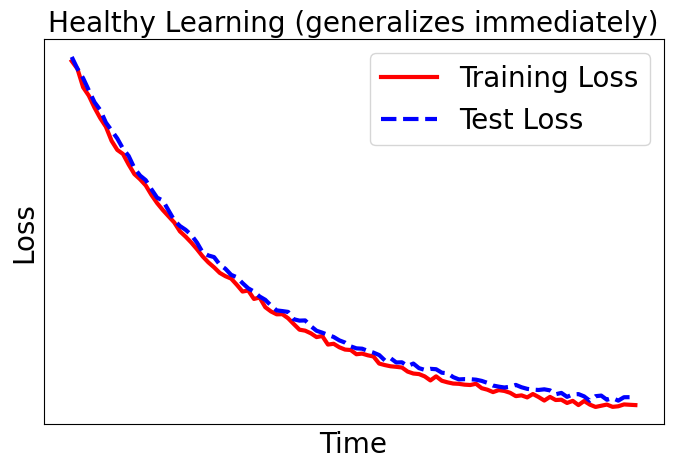
\includegraphics[scale=0.3]{no-grok.png} & 
        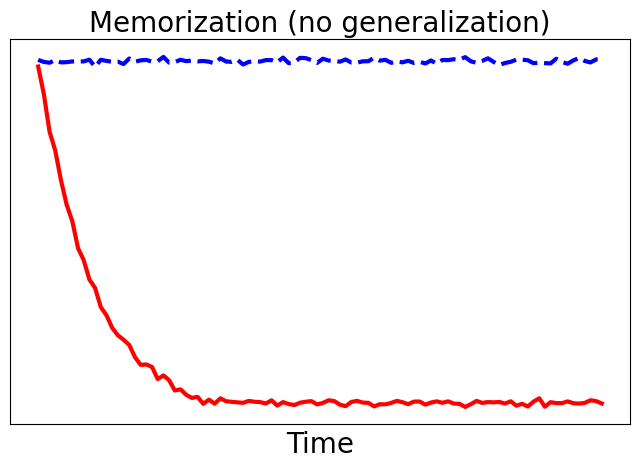
\includegraphics[scale=0.3]{mem.png} &
        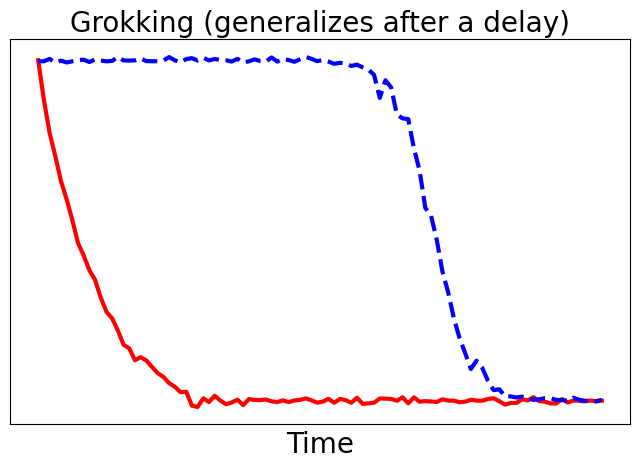
\includegraphics[scale=0.3]{grok.png} \\
        (a) & (b) & (c) \\
    \end{tabular}
    \caption{Healthy learning (a) involves test loss decreasing in-step with training loss. 
    This essentially means that as the model learns about the data it's being trained on, these lessons properly transfer to data it has not been trained on. 
    Under failed learning AKA memorization (b), the test loss never decreases. 
    This failure indicates that the model is memorizing irrelevant qualities of the training data rather than developing a representation capable of generalizing to out-of-distribution data. 
    Grokking (c) involves an initial decrease in train loss followed by a plateau in both, and then a sudden decrease in test loss. 
    Under this dynamic, the model initially memorizes the training dataset and only much later mysteriously learns to generalize to data it has not been trained on.}
    \label{fig:grok}
\end{figure}

In the rapidly evolving landscape of machine learning, the grokking phenomenon presents a unique case of delayed generalization in neural networks, predominantly observed in synthetic datasets under non-optimal hyperparameter settings. 
\textcolor{red}{\cite{liu2023grokking}} and \textcolor{red}{\cite{merrill2023tale}} conceptualize grokking as a form of compression, akin to phase transitions in physical systems, indicating profound shifts in network behavior. 
This interpretation is complemented by the mathematical and algorithmic explorations of \textcolor{red}{\cite{nanda2023progress}} and \textcolor{red}{\cite{rubin2023droplets}}, who illustrate grokking through the lens of emergent problem-solving strategies, diverging from traditional human approaches in tasks like modular arithmetic. 
Further, \textcolor{red}{\cite{liu2022omnigrok, liu2022towards}?} and \textcolor{red}{\cite{kumar2023grokking}} emphasize the role of training dynamics and hyperparameter choices in precipitating grokking, suggesting that this phenomenon is more a consequence of suboptimal network tuning rather than an inherent characteristic of neural learning processes. 
Offering a critical perspective, \cite{pope2023grok} challenges the anthropomorphic implications of the term 'grokking' in the context of machine learning, a sentiment echoed in the alternative interpretations presented by \textcolor{red}{\cite{davies2023unifying}} and \textcolor{red}{\cite{barak2022hidden}}. 
These works collectively underscore the multifaceted nature of grokking, highlighting its potential as both a window into neural network learning dynamics and a topic of ongoing debate in the field.\par
\textcolor{red}{$\uparrow$ this paragraph was written by ChatGPT. i need to do a real one that actually thoroughly reviews the field based on all my notes}

Our primary explanation of the grokking phenomenon will come from \cite{varma2023explaining}, although it could be rewritten in terms of the notation defined in \cite{} as well. \cite{varma2023explaining} essentially posits two distinct possible \textit{circuits} in every model, $C_{mem}$ and $C_{gen}$.
A circuit is just an algorithm, a series of computations that take an input and give a desired output\cite{olah2020zoom}.
The key idea here is that the model can either memorize its training data ($C_{mem}$) or learn a representation of the problem at hand that allows it to generalize to unseen data ($C_{gen}$). 
Neural networks are very good at the former because superposition\cite{elhage2022toy} allows them to store \& compute on a lot of information using a comparatively small number of parameters.
But that still begs the question, \textit{why are they sometimes slower at learning a general representation?}
This is especially puzzling given that $C_{gen}$ is in theory lower dimensional than $C_{mem}$, meaning the former is a smaller, simpler circuit than the latter. 
The two key concepts here are weight decay and dataset size.\par

You may be familiar with weight decay from Bhatt if he ever taught you about simple machine learning.
The L2 Norm as it's called is an additional term added to the loss function (the \textit{goal} of the model, analogous to a utility function in economics).
What it basically does is say "yeah I know your primary goal is great, but here's a thought: what if you tried to accomplish your goal while using as few parameters as possible?"
It basically sums up the squares of the parameters and then penalizes the model for that big number, thereby encouraging it to send as many of its parameters to 0 as possible.\par

So weight decay encourages sparsity, meaning simpler circuits.
And what circuit is simple?
$C_{gen}$ of course.
When a model starts off successfully using $C_{mem}$, thanks to weight decay it will slowly find a bunch of weights inside of it that could \textit{turn into} $C_{mem}$ and grow them while throwing away all of the plethora of weights it used to engage $C_{mem}$.\par

This is the simple explanation. 
The model learns $C_{mem}$ first because it's easier to learn, and then only learns $C_{gen}$ later after encouraged to do so by weight decay.
As to why $C_{gen}$ is harder to learn, it's not always and that has to do with the size of the dataset $D$, but I'm too lazy to get into that rn.
Also there's still a bit of a question as to why grokking can kinda sorta still grokk sometimes even without weight decay.
Rn the hypotheses are that it either has to do with other regularizing components like stochastic gradient descent, or maybe $C_{gen}$ is just slightly more accurate than $C_{mem}$ which is enough for it to eventually surface. \par

That was a long rant to explain grokking but really the key insight here is that $C_{gen}$ should be our new definition of "understanding."
See sources like \cite{tegmark2023spacetime} for why I think it's appropriate to characterize $C_{gen}$ as an actual model of the world, AKA comprehension, while $C_{mem}$ on the other hand is just a bunch of random correlations \`a la stochastic parrots.







\section{Strictly Defining \textit{Computational Comprehension}}
\label{sec:def}

\begin{itemize}
    \item we're going get strict about our definition before analyzing its philosophical merits in section \ref{sec:phil} 
    \item summarize the model of single tasks from \cite{arora2023skills}
    \item simple models that perform single tasks can be said to understand when their test accuracy is high (have grokked or parameters were tuned such that they never needed to grok)
    \item LLMs and other large complex AIs that model many tasks, and therefore do not exhibit any clearly visible grokking in their train/test loss graph, can be said to have slowly built circuits for many individual tasks in such a manner that any grokking is invisible in the train/test curves bc it averages out, or they just had their parameters tuned correctly
    \begin{itemize}
        \item bring up induction heads \cite{olsson2022context} as an example of an early circuit being built in an LLM
        \item cite \cite{brown2020language} when saying that despite smooth decreases in loss, the model exhibits sudden emergent abilities
    \end{itemize}
    \item In theory, a good way to see if an LLM has understood a specific task is to hold back a subset of that task from its training data
    \begin{itemize}
        \item For example, on a shift cypher maybe hold back one or more of the 25 possible shifts from the training data. see \cite{mccoy2023embers}
        \item this would be a hella difficult training dataset to create and I for one have no intention of doing so
    \end{itemize}
\end{itemize}




\section{Why There is No Better Option Philosophically}
\label{sec:phil}

\begin{itemize}
    \item summarize chinese room paradox again
    \item previous philosophers on this subject confuse consciousness and computational circuits. Our argument is that "understanding" can be defined as a low-dimensional/sparse (aka relatively simple, meaning not memorization of the training data) computational circuit that generalizes to unseen examples
    \begin{itemize}
        \item it is possible to "understand" or "know" something without being conscious of it. Likewise, it is possible to be conscious of something without understanding it
        \begin{itemize}
            \item think subconscious knowledge
            \item your brain can have a circuit that allows you to understand something in your memory, and you can be not conscious of it at this given moment
        \end{itemize}
    \end{itemize}
    \item so key here is to stress that we are not actually arguing for/against \href{https://en.wikipedia.org/wiki/Functionalism_(philosophy_of_mind)}{functionalism} or \href{https://en.wikipedia.org/wiki/Computational_theory_of_mind}{computational theory of mind}. Rather, our point is orthogonal; that understanding is in fact computation, and you philosophers can go and continue to squabble on about consciousness. Computational understanding is different from the feeling/qualia of understanding
    \begin{itemize}
        \item \textcolor{red}{might it be good to just always refer to it as "computational understanding" throughout the paper?}
    \end{itemize}
    \item make the case that to argue against us would effectively be to argue for dualism. If this isn't "understanding", then what is? are we conflating consciousness with understanding now?
    \item To hold the standard of "they need to actually \textit{understand} the way I do using qualia within my consciousness" is to demand information that is impossible to gather even if it is true. Furthermore, we don't seem to place the same demand on our fellow humans. We have no proof that our fellow humans are conscious, so how can we know that they understand?
    \item can we find examples of circuits from neuroscience that look similar to our case here?
\end{itemize}


\begin{figure}[h]
    \centering
    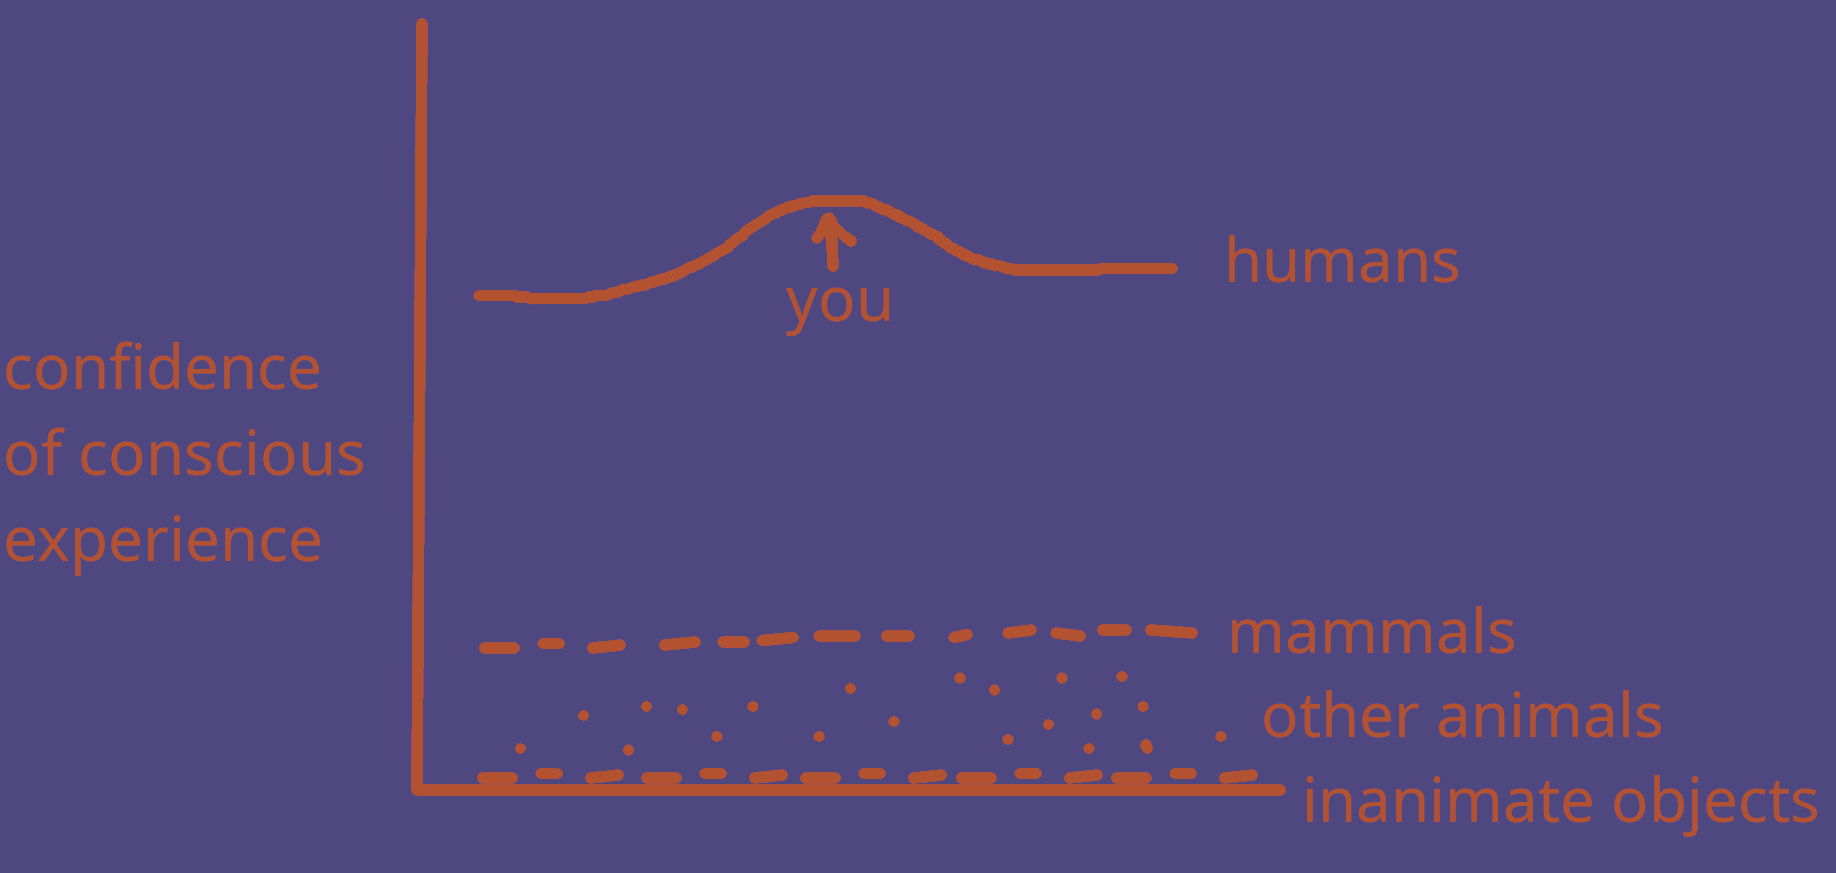
\includegraphics[width=\textwidth]{image.png}
    \caption{You can let this be a log scale (most ppl?), or an exponential scale (borderline/unsure/probabalistic panpsychism)(this is me), or somewhere in-between, or you at 100\% confidence & everything else at zero (full on cogito ergo sum), or everyone at 100\% (100\% panpsychism/nondualism)}
    \label{fig:enter-label}
\end{figure}
idc which scale you use. the consciousness debate is a whole separate one from what we're concerned about in this paper. we are not making claims about consciousness. understanding is a separate thing from consciousness. i can't help you there, i cannot prove that LLMs experience qualia. but u know what? u can't prove that other humans experience qualia. so get fucked. If u think qualia/consciousness is necessary for understanding then you should be unsure that other humans are capable of understanding. that's why it makes sense to allow consciousness and understanding to be separate concepts. You can be conscious of something without understanding it, and you can understand something that you're not conscious of. \par

our current definition of understanding is maybe not the final one. Is it the lowest possible dimensional representation? i don't think so, but certainly a reasonably low one. Our definition of low dimensional representation doesn't conflict with regular computer programs because in those, the "understanding" comes from the coder. That program is essentially performing the Chinese room paradox. In the Chinese room paradox, the correct level of analysis includes the person who wrote all the manuals. In contrast, in deep learning, the understanding does not lie with the programmer. So it's as if we're standing on the outside of the chinese room, the black box appears to act as if it understands, and we know for a fact that there is no person who wrote any manuals. You could say that the learning algorithm understands, or that the data that has been learned off of is what understands, but that's just pushing the problem upstream and doesn't make any sense because the model is the one doing the translating, so it would make more sense to say that the model is the one that understands. Of course this works off of the assumption that in a system, in order to perform an intelligent action, there must be \textit{something} that understands. But by what I just said, wouldn't that imply that there is something in the evolutionary algorithm that understands? yeah. Again i am not saying that the evolutionary algorithm, or an ML algorithm, is conscious. I am not saying that it experiences qualia. I would posit that you do not need to be conscious in order to understand. For example, your subconscious can certainly understand concepts that you are not conscious of, that's the whole point/defintion of a subconscious. Or you can have memories that you can't quite remember at this very moment but will be able to later; maybe they're on the tip of your tongue. Or memories that are not in your conscious experience at this very moment but would be if you were to call them up. Just because you are not conscious of something, just because you are not currently experiencing its corresponding qualia, does not mean that you do not know or understand it. 


\section{Anthropocentric Bias According to this Definition}
\label{sec:anthro}

\begin{itemize}
    \item background on anthropomorphism \& anthropocentric bias
    \item further rephrase claims that models are "just stochastic parrots" in terms of our new grokking definition
\end{itemize}

\begin{table}[h]
 \caption{When Anthropocentrism/morphising Occurs}
  \centering
  \begin{tabular}{l|ll}
     & Model has grokked & Model has not grokked \\
    \midrule
    Human claims model understands & Accurate claim & Anthropomorphizing model \\
    Human claims model does not understand & Anthropocentric bias against model & Accurate claim \\
  \end{tabular}
  \label{tab:2x2table}
\end{table}


\section{Ethical Implications}
\label{sec:ethics}

\begin{itemize}
    \item none if you wanna separate consciousness from understanding
\end{itemize}

\section{Conclusion}
\label{sec:conclusion}
Your conclusion here

\section*{Acknowledgments}
This was was supported in part by......

%Bibliography
\nocite{}
\bibliographystyle{unsrt}  
\bibliography{references}  

\end{document}
